\documentclass[11pt,xcolor={dvipsnames},aspectratio=159,hyperref={pdftex,pdfpagemode=UseNone,hidelinks,pdfdisplaydoctitle=true},usepdftitle=false]{beamer}
\usepackage{presentation}[aspectratio=169]
\usepackage{math}
\usepackage{mathtools}
\usepackage{mleftright}
\usepackage{algorithm}% http://ctan.org/pkg/algorithms
\usepackage{algpseudocode}% http://ctan.org/pkg/algorithmicx
\hypersetup{
    colorlinks=magenta,
    linkcolor=magenta,
    filecolor=magenta,      
    urlcolor=magenta,
    }
% Enter title of presentation PDF:
\hypersetup{pdftitle={Equations}}


\begin{document}
% Enter presentation title:
\title{Solving Equations}
\subtitle{Quantitative Economics 2024}
% Enter presentation information:

% Enter presentation authors:
\author{Piotr Żoch}%
% Enter presentation location and date (optional; comment line if not needed):
\frame{\titlepage}

% Fill out content of presentation:
\begin{frame}{Introduction}   
\begin{itemize}
    \item Systems of linear equations.
    \item Nonlinear equations.
\end{itemize}
\end{frame}


\begin{frame}
    \heading{Linear equations}
    \end{frame}

\begin{frame}{Linear systems of equations}
    \begin{itemize}
        \item One of the most common problems in scientific computation: solve  
\begin{align*}
    \mathbf{A}\mathbf{x} = \mathbf{b},
\end{align*}
for $\mathbf{x}$, where $\mathbf{A}$ is a square matrix and $\mathbf{b}$ is a vector.
    \item Seems like an easy problem, but it will teach us many things.
    \item Multiple specialized libraries for numerical linear algebra.
\end{itemize}
\end{frame}

\begin{frame}{Direct methods}
    \begin{itemize}
        \item Elementary operations: 
        \begin{itemize}
            \item mutliply a row by a scalar,
            \item add a scalar multiple of a row to another row,
            \item interchange two rows. 
        \end{itemize}
        \item Solve $\mathbf{A}\mathbf{x} = \mathbf{b}$ by using elementary row operations on the augmented matrix $[\mathbf{A}\mid\mathbf{b}]$.
        \item Transform $\mathbf{A}$ into a reduced row echelon form. 
    \end{itemize}
    \end{frame}


\begin{frame}{Direct methods}
    \begin{itemize}
        \item Two step procedure:
        \begin{itemize}
            \item Forward elimination. \begin{align*} \scriptsize
                \left[\begin{array}{cccc|c}
                    * & * & * & * & * \\
                    * & * & * & * & * \\
                    * & * & * & * & * \\
                    * & * & * & * & * \\
                    \end{array}\right]
                    \rightarrow
                    \left[\begin{array}{cccc|c}
                        * & * & * & * & * \\
                          & * & * & * & * \\
                          & * & * & * & * \\
                          & * & * & * & * \\
                    \end{array}\right]  
                    \rightarrow
                    \left[\begin{array}{cccc|c}
                        * & * & * & * & * \\
                         & * & * & * & * \\
                         &  & * & * & * \\
                         &  & * & * & * \\
                    \end{array}\right]
                    \rightarrow
                    \left[\begin{array}{cccc|c}
                        * & * & * & * & * \\
                         & * & * & * & * \\
                         &  & * & * & * \\
                         &  &   & * & * \\
                    \end{array}\right]                  
            \end{align*}
            \item Backward elimination. \begin{align*} \scriptsize
            \left[\begin{array}{cccc|c}
                * & * & * & * & * \\
                 & * & * & * & * \\
                 &  & * & * & * \\
                 &  &   & * & * \\
            \end{array}\right] 
                    \rightarrow
            \left[\begin{array}{cccc|c}
                * & * & * &  & * \\
                 & * & * &  & * \\
                 &  & * &  & * \\
                 &  &   & * & * \\
            \end{array}\right] 
                    \rightarrow
                    \left[\begin{array}{cccc|c}
                        * & * &  &  & * \\
                         & * &  &  & * \\
                         &  & * &  & * \\
                         &  &   & * & * \\
                    \end{array}\right] 
                    \rightarrow
                    \left[\begin{array}{cccc|c}
                        * &  &  &  & * \\
                         & * &  &  & * \\
                         &  & * &  & * \\
                         &  &   & * & * \\
                    \end{array}\right] 
            \end{align*}
        \end{itemize}
    \end{itemize}
    \end{frame}
    

\begin{frame}{Floating point numbers}

    \begin{itemize}  
    \item Forward elimination: to deal with the first column we need $n^2$ operations, for the second $n^2 - 1$, for the third $n^2 - 2$ and so on.
    \item Backward elimination: to deal with the last column we need $n$ operations, for the second to last $n-1$, for the third to last $n-2$ and so on.
    \item Forward elimination is $\Oc\of{n^3}$, backward elimination is $\Oc\of{n^2}$.
    \end{itemize}
    \end{frame}

\begin{frame}{Triangular systems}
    \begin{itemize}  
    \item Lower triangular system: 
        \begin{align*}
        \begin{bmatrix}
            1 & 0 & 0 & 0 \\
            l_{21} & 1 & 0 & 0 \\
            l_{31} & l_{32} & 1 & 0 \\
            l_{41} & l_{42} & l_{43} & 1
        \end{bmatrix}
        \begin{bmatrix}
            y_1 \\
            y_2 \\
            y_3 \\
            y_4
        \end{bmatrix}
        =
        \begin{bmatrix}
            b_1 \\
            b_2 \\
            b_3 \\
            b_4
        \end{bmatrix}
        \end{align*}
        can be solved using forward elimination, starting from the top
        \begin{align*}
            y_i = b_i - \sum_{j=1}^{i-1} l_{ij} y_j.
        \end{align*}
\end{itemize}
\end{frame}

\begin{frame}{Upper triangular systems}
    \begin{itemize}  
    \item Upper triangular system: 
        \begin{align*}
        \begin{bmatrix}
            u_{11} & u_{12} & u_{13} & u_{14} \\ 
            0 & u_{22} & u_{23} & u_{24} \\ 
            0 & 0 & u_{33} & u_{34} \\ 
            0 & 0 & 0 & u_{44}
        \end{bmatrix}
        \begin{bmatrix}
            x_1 \\ 
            x_2 \\ 
            x_3 \\ 
            x_4
        \end{bmatrix}
        =
        \begin{bmatrix}
            y_1 \\ 
            y_2 \\ 
            y_3 \\ 
            y_4
        \end{bmatrix}
        \end{align*}
        can be solved using backward elimination, starting from the bottom
        \begin{align*}
            x_i = \frac{1}{u_{ii}}\bp{y_i - \sum_{j=i+1}^{n} u_{ij} x_j}.
        \end{align*}
    \end{itemize}
\end{frame}

\begin{frame} 
\begin{itemize} 
    \item Suppose we can write \begin{align*}
        \mathbf{A} = \mathbf{L} \mathbf{U}
    \end{align*}
    where $\mathbf{L}$ is a lower triangular matrix and $\mathbf{U}$ is an upper triangular matrix.
    \item We have \begin{align*}
        \mathbf{L} \bp{\mathbf{U} \mathbf{x}}   = \mathbf{b} \rightarrow \mathbf{L} \mathbf{y}  = \mathbf{b}
    \end{align*}
    which we can solve for $\mathbf{y}$ using forward elimination.
    \item  We then solve \begin{align*}
        \mathbf{U} \mathbf{x} = \mathbf{y}
    \end{align*}
    for $\mathbf{x}$ using backward elimination.
\end{itemize}
\end{frame}

\begin{frame} 
    \begin{itemize} 
        \item This is known as Gaussian elimination.
        \begin{enumerate}
        \item Compute $\mathbf{L}$ and $\mathbf{U}$.
        \item Solve $\mathbf{L} \mathbf{y} = \mathbf{b}$ for $\mathbf{y}$ using forward elimination.
        \item Solve $\mathbf{U} \mathbf{x} = \mathbf{y}$ for $\mathbf{x}$ using backward elimination.
        \end{enumerate}
        \item Step 1. is known as \al{LU decomposition}.
        \item Nice thing: we can keep $\mathbf{L}$ and $\mathbf{U}$ and recycle them for different $\mathbf{b}$.
        \item How to perform the decomposition?
    \end{itemize}
    \end{frame}


\begin{frame}{Matrix multiplication by outer products}
\begin{itemize}
    \item Write the columns of $\mathbf{A}$ as $\mathbf{a}_1, \ldots, \mathbf{a}_n$.
    \item Write the rows of $\mathbf{B}$ as $\mathbf{b}^\intercal_1, \ldots, \mathbf{b}^\intercal_n$.
    \item We have \begin{align*}
        \mathbf{A}\mathbf{B} = \sum_{k=1}^n \mathbf{a}_k \mathbf{b}^\intercal_k.
    \end{align*}
    \item Useful: for triangular matrices $\mathbf{L},\mathbf{U}$ only the first outer product contributes to the first row and the first column of $\mathbf{L} \mathbf{U}$
    \begin{align*}
        \mathbf{e}^\intercal_1 \sum_{k=1}^n \mathbf{l}_k \mathbf{u}^\intercal_k = l_{11} \mathbf{u}^\intercal_1, \quad \bp{\sum_{k=1}^n \mathbf{l}_k \mathbf{u}^\intercal_k} \mathbf{e}_1 = u_{11} \mathbf{l}_1.
    \end{align*}
\end{itemize}

\end{frame}

\begin{frame}{LU Factorization without Pivoting}
    \begin{algorithm}[H]
        \scriptsize
        \caption{LU Factorization without Pivoting}
        \begin{algorithmic}[1]
            \Require Matrix $\mathbf{A} \in \mathbb{R}^{n \times n}$
                \For{$j = 1$ to $n$}
                \For{$i = j+1$ to $n$}
                    \State $a_{ij} = \frac{a_{ij}}{a_{jj}}$
                    \For{$k = j+1$ to $n$}
                        \State $a_{ik} = a_{ik} - a_{ij} a_{jk}$
                    \EndFor
                \EndFor
            \EndFor
        \end{algorithmic}
    \end{algorithm}
\begin{itemize} 
    \item This algorithm uses $\mathbf{A}$ matrix to store $\mathbf{L}$ and $\mathbf{U}$.
    \item Problem when $a_{jj} = 0$ at any step - 
\end{itemize}
\end{frame}
\begin{frame}{Solving the system}
   \begin{itemize}
   \item We need \begin{align*}
    \sum_{j=1}^n \sum_{i=j+1}^n \bp{1+\sum_{k=j+1}^n 2} = \frac{2}{3} n^3 - \frac{1}{2}n^2 - \frac{1}{6}n
   \end{align*}
    operations to perform the factorization.
    \item We then need \begin{align*}
        \sum_{i=1}^n \bp{2+\sum_{j=1}^{i-1} 2 } = n^2 + n
    \end{align*}
    operations for forward and backward substitution each. 
    \item LU decomposition is the most costly step. 
\end{itemize}
\end{frame}


\begin{frame}{Solving the system}
   \begin{itemize}
   \item We need \begin{align*}
    \sum_{j=1}^n \sum_{i=j+1}^n \bp{1+\sum_{k=j+1}^n 2} = \frac{2}{3} n^3 - \frac{1}{2}n^2 - \frac{1}{6}n
   \end{align*}
    operations to perform the factorization.
    \item We then need \begin{align*}
        \sum_{i=1}^n \bp{2+\sum_{j=1}^{i-1} 2 } = n^2 + n
    \end{align*}
    operations for forward and backward substitution each. 
    \item LU decomposition is the most costly step. 
\end{itemize}
\end{frame}

\begin{frame}{Solving the system}
    \begin{itemize}
    \item In practice we use a similar method, but with \alg{pivoting}
    \item PLU factorization: \begin{align*}
        \tilde{\mathbf{A}} = \mathbf{L} \mathbf{U},
    \end{align*}
    where $\tilde{\mathbf{A}}$ is a matrix $\mathbf{A}$ with its rows permuted.
    \item It works if and only if $\mathbf{A}$ is non-singular.
    \item Asymptotically uses the same number of operations and LU without pivoting.
\end{itemize}
\end{frame}


\begin{frame}{Norms}
    \begin{itemize}
    \item A \alg{vector norm} is a function $\norm{\cdot}:\mathbb{R}^n \rightarrow \mathbb{R}$ that satisfies:
    \begin{enumerate}
        \item $\norm{\mathbf{x}} \geq 0$,
        \item $\norm{\mathbf{x}} = 0 \iff \mathbf{x} = \mathbf{0}$,
        \item $\norm{a\mathbf{x}} = |a|\norm{\mathbf{x}}$,
        \item $\norm{\mathbf{x} + \mathbf{y}} \leq \norm{\mathbf{x}} + \norm{\mathbf{y}}$,
    \end{enumerate}
    for all $\mathbf{x},\mathbf{y} \in \mathbb{R}^n$ and $a \in \mathbb{R}$.
    \item Common vector norms: $\ell_1$, $\ell_2$, $\ell_\infty$: \begin{align*}
        \norm{\mathbf{x}}_1 = \sum_{i=1}^n |x_i|, \quad \norm{\mathbf{x}}_2 = \sqrt{\sum_{i=1}^n x_i^2}, \quad \norm{\mathbf{x}}_\infty = \max_{i=1,\ldots,n} |x_i|.\end{align*}
\end{itemize}
\end{frame}


\begin{frame}{Norms}
    \begin{itemize}
    \item For matrices we have \alg{matrix norms}.
    \item A \al{Frobenius} norm is \begin{align*}
        \norm{\mathbf{A}}_F = \sqrt{\sum_{i=1}^m \sum_{j=1}^n a_{ij}^2}.
    \end{align*}
    \item Imagine representing a matrix as a vector with columns stacked on top of each other.
    \item An \alb{induced} matrix norm is \begin{align*}
        \norm{\mathbf{A}}_p = \max_{\norm{\mathbf{x}}_p = 1} \norm{\mathbf{A}\mathbf{x}}_p.
    \end{align*}
    \item In Julia: \texttt{norm(A)} is the Frobenius norm, \texttt{opnorm(A,p)} is the induced norm.
\end{itemize}
\end{frame}

\begin{frame}{Norms}
    \begin{itemize}
    \item We have \begin{enumerate}
    \item $\norm{\mathbf{A \mathbf{x}}} \leq \norm{\mathbf{A}} \norm{\mathbf{x}}$, 
        \item $\norm{\mathbf{A} \mathbf{B}} \leq \norm{\mathbf{A}}  \norm{\mathbf{B}}$,
        \item for a square matrix, $\norm{\mathbf{A}^k} \leq \norm{\mathbf{A}}^k$ for any integer $k\geq0$.
    \end{enumerate}
    \item Two common matrix norm are the \al{1-norm} and the \al{$\infty$-norm}:
    \begin{align*}
        \norm{\mathbf{A}}_1 = \max_{j=1,\ldots,n} \sum_{i=1}^m |a_{ij}|, \quad \norm{\mathbf{A}}_\infty = \max_{i=1,\ldots,m} \sum_{j=1}^n |a_{ij}|.\end{align*}
\end{itemize}
\end{frame}


\begin{frame}{Conditioning of linear systems}
    \begin{itemize} 
        \item Consider the perturbed system \begin{align*}
            \mathbf{A}\bp{ \mathbf{x}+ \mathbf{h}}  = \mathbf{b} + \mathbf{d}. \end{align*}
            \item The condition number is the relative change in the solution divided by the relative change in the data: \begin{align*}
                \kappa = \frac{\norm{\mathbf{h}}/\norm{\mathbf{x}}}{\norm{\mathbf{d}}/\norm{\mathbf{b}}} = \frac{\norm{\mathbf{h}}\norm{\mathbf{b}}}{\norm{\mathbf{d}}\norm{\mathbf{x}}}.
            \end{align*}
            \item Note that $\mathbf{h} = \mathbf{A}^{-1} \mathbf{d}$ so \begin{align*}
                \norm{\mathbf{h}} \leq \norm{\mathbf{A}^{-1}} \norm{\mathbf{d}}.
            \end{align*}
            \end{itemize}
\end{frame}


\begin{frame}{Conditioning of linear systems}
    \begin{itemize} 
        \item Use $\norm{\mathbf{h}} \leq \norm{\mathbf{A}^{-1}} \norm{\mathbf{d}}$ to write   \begin{align*}
            \frac{\norm{\mathbf{h}}\norm{\mathbf{b}}}{\norm{\mathbf{d}}\norm{\mathbf{x}}} \leq \frac{\norm{\mathbf{A}^{-1}}\norm{\mathbf{d}}\norm{\mathbf{A}}\norm{\mathbf{x}}}{\norm{\mathbf{d}}\norm{\mathbf{x}}} = \norm{\mathbf{A}^{-1}}\norm{\mathbf{A}}.
            \end{align*}
        \item We can prove that inequality is tight.
        \item The matrix \al{condition number} of an invertible square matrix $\mathbf{A}$ is $$\kappa\bp{\mathbf{A}} = \norm{\mathbf{A}^{-1}}\norm{\mathbf{A}}.$$
            \end{itemize}
\end{frame}


\begin{frame}{Conditioning of linear systems}
    \begin{itemize} 
        \item If $\mathbf{A}\bp{\mathbf{x} +\Delta \mathbf{ x}} = \mathbf{b} + \Delta \mathbf{b}$ then \begin{align*}
        \frac{\norm{\Delta \mathbf{x}}}{\norm{\mathbf{x}}} \leq \kappa\bp{\mathbf{A}} \frac{\norm{\Delta \mathbf{b}}}{\norm{\mathbf{b}}}.
            \end{align*}
        \item The condition number is a measure of how sensitive the solution is to changes in the data.
        \item We can derive a similar result for perturbed $\mathbf{A}$.
        \item The condition number is at least equal to 1.
        \item A condition number of $10^k$ means that we lose $k$ digits of precision.
            \end{itemize}
\end{frame}

\begin{frame}{Conditioning of linear systems}
    \begin{itemize} 
        \item Suppose that we compute a "solution" $\tilde{\mathbf{x}}$ to the system $\mathbf{A}\mathbf{x} = \mathbf{b}$.
        \item We would like to compare $\tilde{\mathbf{x}}$ to the true solution $\mathbf{x}$ - but we do not know $\mathbf{x}$.
        \item We can calculate the \al{residual} $$\mathbf{r} = \mathbf{b} - \mathbf{A}\tilde{\mathbf{x}}$$.
        \item We have \begin{align*}
        \frac{\norm{\mathbf{x} - \tilde{\mathbf{x}}}}{\norm{\mathbf{x}}} \leq \kappa\bp{\mathbf{A}} \frac{\norm{\mathbf{r}}}{\norm{\mathbf{b}}}.
        \end{align*}
        \end{itemize}
\end{frame}

\begin{frame}{Iterative methods}
    \begin{itemize}
    \item We saw that Gaussian elimination is $\Oc\of{n^3}$.
    \item This is prohibitive for large $n$ (unless a matrix has a special structure).
    \item But matrix-vector multiplication is $\Oc\of{n^2}$.
    \item In some cases we can apply repeated matrix-vector multiplication to solve the system.
    \item We call these \alg{iterative methods}.
    \end{itemize}
\end{frame}
    \begin{frame}{Jacobi method}
\begin{itemize}
\item Suppose we want to solve $\mathbf{A}\mathbf{x} = \mathbf{b}$.
\item This can be written as \begin{align*}
    \sum_{j=1}^n a_{ij} x_j = b_i, \quad \text{or} \quad   x_i = \frac{1}{a_{ii}}\bp{b_i - \sum_{j\neq i} a_{ij} x_j}.
\end{align*} 

\item Start from some initial $\mathbf{x}^{(0)}$ and iterate: \begin{align*}
    x_i^{(k+1)} = \frac{1}{a_{ii}}\bp{b_i - \sum_{j\neq i} a_{ij} x_j^{(k)}} 
\end{align*}
until $\mathbf{x}^{(k+1)}$ is close enough to $\mathbf{x}^{(k)}$.
\end{itemize}
\end{frame}


\begin{frame}{Gauss-Seidel method}
\begin{itemize}
    \item We can also write \begin{align*}
        x_i = \frac{1}{a_{ii}}\bp{b_i - \sum_{j=1}^{i-1} a_{ij} x_j - \sum_{j=i+1}^n a_{ij} x_j}.
    \end{align*}
    \item The Gauss-Seidel method uses the newest values of $x_j$: 
    \begin{align*}
        x_i^{(k+1)} = \frac{1}{a_{ii}}\bp{b_i - \sum_{j=1}^{i-1} a_{ij} x_j^{(k+1)} - \sum_{j=i+1}^n a_{ij} x_j^{(k)}}.
    \end{align*}
\end{itemize}
\end{frame}

\begin{frame}{Iterative methods}
    \begin{itemize}
        \item Rewrite $\mathbf{A} = \mathbf{P} - \mathbf{N}$ so that the system is \begin{align*}
            \mathbf{P}\mathbf{x} = \mathbf{N}\mathbf{x} + \mathbf{b}.
        \end{align*} 
        \item An iterative method is \begin{align*}
            \mathbf{P} \mathbf{x}^{(k+1)} = \bp{\mathbf{N}\mathbf{x}^{(k)} + \mathbf{b}}.
        \end{align*}
        \item $\mathbf{P}$ is called a \alg{preconditioner}
        \item Jacobi and Gauss-Seidel differ in the choice of $\mathbf{P}$.
        \item Since $\mathbf{x}^{{k+1}} = \mathbf{P}^{-1}\bp{\mathbf{N}\mathbf{x}^{(k)} + \mathbf{b}}$ a good preconditioner should be easy to invert.
    \end{itemize}
    \end{frame}
    
    \begin{frame}{Iterative methods}
        \begin{itemize}
            \item Why do we call $\mathbf{P}$ a preconditioner?
            \item Suppose we have a system $\mathbf{A}\mathbf{x} = \mathbf{b}$.
            \item The condition number is $\kappa\bp{\mathbf{A}}$.
            \item Suppose we have a preconditioned system $\mathbf{P}^{-1}\mathbf{A}\mathbf{x} = \mathbf{P}^{-1}  \mathbf{b}$.
            \item The condition number is $\kappa\bp{\mathbf{P}^{-1}\mathbf{A}}$.
            \item If $\mathbf{P}\approx\mathbf{A}^-1$, then $\kappa\bp{\mathbf{P}^{-1}\mathbf{A}} \approx 1$.
        \end{itemize}
        \end{frame}
        
    \begin{frame}{Iterative methods}
        \begin{itemize}
            \item Iterative methods do not always converge.
            \item They are guaranteed to converge if $\mathbf{A}$ is \alg{diagonally dominant}: \begin{align*}
                |a_{ii}| > \sum_{j\neq i} |a_{ij}|. \end{align*}
                \item There are better methods than Jacobi and Gauss-Seidel - the idea is to choose $\mathbf{P}$ so that the convergence is faster.
            \end{itemize}

        \end{frame}
        
    \begin{frame}
        \heading{Nonlinear equations}
        \end{frame}

    \begin{frame}{Nonlinear equations}
      
        \begin{itemize}
        
            \item We want to find a solution $x^*$ to 
    \begin{align*}
       f\of{x} = 0.
    \end{align*}
    \item We call $x^*$ a \alg{root} of $f$.
    \item Usually we cannot get the exact solution in a finite number of steps. 
    \item We will focus on $f:\mathbb{R} \rightarrow \mathbb{R}$.
    \item Even simple polynomial equations can have no \al{closed-form} solution: \begin{align*}
        x^5 + 2x^2  + 1= 0.
    \end{align*}
\end{itemize}
    \end{frame}

    \begin{frame}{Bisection method}
      
        \begin{itemize}
        
            \item Suppose we have a continuous function $f:\mathbb{R} \rightarrow \mathbb{R}$.
            \item We do not require it to be differentiable.
            \item We also have two points $a<b$ such that $f\of{a}f\of{b} < 0$ (opposite signs).
            \item We call $\bs{a,b}$ a \alg{bracket}. 
            \item By the \alg{intermediate value theorem} there exists a point $x^*$ such that $f\of{x^*} = 0$, $x^* \in \bp{a,b}$.
            \item Evaluate $f\of{m}$ where $m = \frac{a+b}{2}$. 
            \begin{itemize}
                \item If $f\of{m} = 0$ we are done.
                \item If $f\of{m}f\of{a} < 0$ then $x^* \in \bp{a,m}$. Use $m$ as the new $b$.
                \item If $f\of{m}f\of{b} < 0$ then $x^* \in \bp{m,b}$. Use $m$ as the new $a$.
            \end{itemize}
            \item Repeat until $b-a$ is small enough.
\end{itemize}
    \end{frame}

\begin{frame}{Bisection method}
    \begin{figure}    
    \centering
        
        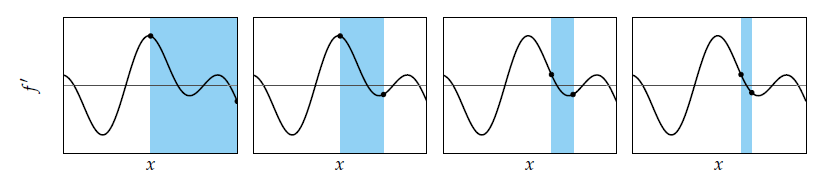
\includegraphics[width=1\textwidth]{bisection.png}
        \caption{Source: \href{https://mitpress.mit.edu/9780262039420/}{Kochenderfer and Wheeler (2019). Note: $f'$ corresponds to our $f$.}}
        \end{figure}
    \end{frame}
    

\begin{frame}{Bisection method}
    
    \begin{itemize}
    
        \item \alg{Good}: bisection is \emph{guaranteed} to converge to a root.
        \item \alr{Bad}: it is slow. But how slow? 
        \item If there are multiple roots, it will find just one of them -- this is a general problem with root-finding algorithms.        

\end{itemize}
\end{frame}

\begin{frame}{Convergence}
    
    \begin{itemize}
        \item A sequence $\bc{x_1,x_2,\ldots}$ converges to $x^*$ with \alb{order $p$}, if there exists a constant $C$ such that \begin{align*}
            \abs{x_{k+1} - x^*} \leq r \abs{x_k - x^*}^p.
        \end{align*}
        for all $k$ large enough.
        \item We call $r$ the \al{rate of convergence}. 
        \item A method is locally convergent if the sequence converges to $x^*$ for $x_0$ close enough to $x^*$.
        \item A method is globally convergent if the sequence converges to $x^*$ for any $x_0$.
\end{itemize}
\end{frame}

\begin{frame}{Bisection method}
    
    \begin{itemize}
        \item The initial bracket in the bisection method is $I_0 = \bs{a,b}$. Its length is $b-a$.
        \item The bracket after the first iteration is either $I_1 = \bs{a,\frac{a+b}{2}}$ or $I_1 = \bs{\frac{a+b}{2},b}$. Its length is $\frac{b-a}{2}$.
        \item The bracket after the $k$-th iteration has length $\frac{b-a}{2^k}$.
        \item We have \begin{align*}
            \abs{x_k - x^*} \leq \bp{\frac{1}{2}}  \abs{x_{k-1} - x^*}
        \end{align*}
        \item The order of convergence is $p=1$ and the rate of convergence is $r = \frac{1}{2}$.
\end{itemize}
\end{frame}


\begin{frame}{Bisection method}
    
    \begin{itemize}
        \item We add one bit of precision in each iteration.
        \item To get one digit of precision we need to perform $\approx 3.3$ iterations (since $\log_2 10 \approx 3.3$).
        \item If we want to have $\abs{x^k - x^*} \leq \gamma$, we need to perform $$k=\log_2\bp{\frac{\abs{b-a}}{\gamma}}$$ iterations. 
        \item The above follows from $$\abs{x^k - x^*} \leq 2^{-k}\abs{b-a}.$$
\end{itemize}
\end{frame}

\begin{frame}{Bisection method}
    
    \begin{itemize}
        \item Bisection has $p=1$ and $r=\frac{1}{2}$. If $p=1$ and $r<1$ the order of convergence is called \al{linear}.
        \item If $p=1$ but $r_k$<1 and $r_k\rightarrow 0 $ as $k\rightarrow \infty$ the order of convergence is called \al{superlinear}.
        \item If $p=2$ the order of convergence is called \al{quadratic}.
        \item If $p=3$ the order of convergence is called \al{cubic}...
        \item The order of convergence does not have to be an integer.
\end{itemize}
\end{frame}



\begin{frame}{Newton method}
    
    \begin{itemize}
        \item The bisection method did not use much information about the function $f$.
        \item We can use more information to design faster methods.
        \item Consider a Taylor expansion of $f\of{x^*}$ around $x$: \begin{align*}
            f\of{x^*} = f\of{x} + f'\of{x}\bp{x^*-x} + \frac{1}{2}f''\of{\xi}\bp{x^*-x}^2, \quad \xi\in\bp{x^*,x}   \end{align*}
        \item Use $f\of{x^*}=0$ to solve for $x^*$:
            \begin{align*}
                x^* = x - \frac{f\of{x}}{f'\of{x}} + o\of{\abs{x^*-x}}.
            \end{align*}
        \item This suggests that $x^*$ is close to $x - \frac{f\of{x}}{f'\of{x}}$.
\end{itemize}
\end{frame}

\begin{frame}{Newton method}
    
    \begin{itemize}
        \item Start with $x_0$ and consider the sequence given by $$x_{k+1} = x_k -\frac{f\of{x_k}}{f'\of{x_k}}.$$
        \item This is the \alg{Newton method}. Also known as the \alg{Newton-Raphson method}.
        \item Be careful: the method can diverge. Easy to see if $f'\of{x} = 0$.
\end{itemize}
\end{frame}


\begin{frame}{Newton method}
    
    \begin{itemize}
        \item What is the order of convergence of the Newton method? 
        \item We have $x_k = x^* + e_k$, where $e_k$ is the error at the $k$-th iteration.
        \item We have \begin{align*}
            e_{k+1} &= e_k - \frac{f\of{x_k}}{f'\of{x_k}} \\
            &= e_k - \frac{f\of{x^* + e_k}}{f'\of{x^* + e_k}} \\
            &= \frac{\frac{1}{2}f''\of{x^*}e_k^2 + \frac{1}{3}f'''\of{x^*}\bp{e_k^3 + o\of{e_k^3}}}{f'\of{x^*} + f''\of{x^*}e_k^2 + o\of{e_k}} \\
            &= \frac{f''\of{x^*}}{2f'\of{x^*}}e_k^2 + o\of{e_k^2}, 
        \end{align*}
        if $f''\of{x^*} \neq 0$. Note that $e_k$ is raised to the power of 2.
\end{itemize}
\end{frame}

\begin{frame}{Newton method}
    
    \begin{itemize}
        \item The order of convergence is $p=2$, so it is \alb{quadratic}.
        \item The number of correct digits approximately doubles in each iteration.
        \item Good guess: 6-7 iterations to get an answer within machine precision. 
        \item Note: if $x^*$ is a double root, then $e_{k+1} \approx \frac{1}{2} e_k$ - linear convergence.
\end{itemize}
\end{frame}

\begin{frame}{Newton method}
    
    \begin{itemize}
        \item \alg{Good}: the Newton method is fast.
        \item \alr{Bad}: you need a good guess, not guaranteed to converge. 
        \item You also need to calculate the derivative at each $x_k$. How to do this? 
        \item $f$ has to be sufficiently smooth (we used the Taylor expansion to show quadratic convergence).
    \end{itemize}
\end{frame}

\begin{frame}{Secant method}
    
    \begin{itemize}
        \item Insteady of calculating the derivative, we can approximate it.
        \item Suppose we have two points $x_k$ and $x_{k-1}$.
        \item We can approximate the derivative at $x_k$ as \begin{align*}
            f'\of{x_k} \approx \frac{f\of{x_k} - f\of{x_{k-1}}}{x_k - x_{k-1}}. \end{align*}
        \item The secant method is \begin{align*}
            x_{k+1} = x_k - f\of{x_k}\frac{x_k - x_{k-1}}{f\of{x_k} - f\of{x_{k-1}}}.
        \end{align*}
        \item The order of convergence is $p\approx 1.6$.
        \item Requires two initial guesses.
    \end{itemize}
\end{frame}

\begin{frame}{Secant method}
    
    \begin{itemize}
        \item $p\approx 1.6$ is between linear and quadratic convergence. Seems worse than Newton.
        \item In each iteration of Newton we use $f'\of{x_k}$ and $f\of{x_k}$.
        \item In each iteration of the secant method we use $f\of{x_k}$ and $f\of{x_{k-1}}$, but we already calculated $f\of{x_{k-1}}$ in the previous iteration.
        \item If function evaluations are used to measure computational work, the secant iteration converges more rapidly than Newton's method.
    \end{itemize}
\end{frame}

\begin{frame}{Brent method}
    
    \begin{itemize}
        \item Bisection is slow, but guaranteed to converge.
        \item Newton is fast, but requires a good guess.
        \item The \alg{Brent method} (Dekker-Brent) combines the two: \begin{enumerate}
            \item Start with a bracket. 
            \item Do a step of Newton / secant to get $x_k$. If it is within the bracket, accept it. Otherwise do bisection.
            \item Update the bracket using the new point. 
            \item Repeat until convergence. 
        \end{enumerate}
        \item The Brent method uses an inverse quadratic interpolation to get an approximate $f'$.
    \end{itemize}
\end{frame}


\begin{frame}{Multidimensional methods}
    
    \begin{itemize} 
    \item Newton's method can be extended to multiple dimensions; $f:\mathbb{R}^n \rightarrow \mathbb{R}^n$.
    \item Suppose we want to solve $\mathbf{f}\of{\mathbf{x}} = \mathbf{0}$.
    \item The Newton method is \begin{align*}
        \mathbf{x}_{k+1} = \mathbf{x}_k - \bs{\mathbf{J}\of{\mathbf{x}_k}}^{-1} \mathbf{f}\of{\mathbf{x}_k}.
\end{align*}
\item $\mathbf{J}$ is the Jacobian matrix of $f$: \begin{align*}
    \mathbf{J}_{ij}\of{\mathbf{x}} = \frac{\partial \mathbf{f}_i\of{\mathbf{x}}}{\partial x_j}.
\end{align*}
\end{itemize}
\end{frame}

\begin{frame}{Multidimensional methods}
    
    \begin{itemize} 
    \item In practice we do not calculate the inverse of the Jacobian.
    \item We solve \begin{align*}
        \mathbf{J}\of{\mathbf{x}_k}\mathbf{s}_k = -\mathbf{f}\of{\mathbf{x}_k}.
    \end{align*}
    and update \begin{align*}
        \mathbf{x}_{k+1} = \mathbf{x}_k + \mathbf{s}_k. 
    \end{align*}
    \item Challenge: it is expensive to calculate the Jacobian.
\end{itemize}
\end{frame}


\begin{frame}{Broyden method}
    
    \begin{itemize} 
    \item Note that what we do is: \begin{align*}
        \mathbf{A}_k \mathbf{s}_k & = -\mathbf{f}\of{\mathbf{x}_k}. \\
        \mathbf{x}_{k+1}  & = \mathbf{x}_k + \mathbf{s}_k. 
    \end{align*}
\item We had $\mathbf{A}_k = \mathbf{J}\of{\mathbf{x}_k}$. But there are other ways to choose $\mathbf{A}_k$.
\item One possible choice is \begin{align*}
    \mathbf{A}_{k+1} = \mathbf{A}_k + \frac{1}{\mathbf{s}_k^\intercal \mathbf{s}_k}\bs{\mathbf{f}\of{\mathbf{x}_{k+1}} - \mathbf{f}\of{\mathbf{x}_{k}} - \mathbf{A}_k \mathbf{s}_k }\mathbf{s}^\intercal_k. \end{align*}
\item This is the \alg{Broyden method}.
\item Under some conditions the Broyden method converges superlinearly (but $\mathbf{A}_k$ is not guaranteed to converge to the Jacobian).
\end{itemize}
\end{frame}

\begin{frame}{Levenberg step}
    
    \begin{itemize} 
\item Problem: it is possible to diverge.
\item One way to prevent divergence is to add a \alg{Levenberg step}.
\item Check if an usual Newton step would lead to an improvement.
\item If not, go in a direction that is guaranteed to an improvement.
\begin{align*}
\bp{\mathbf{A}^\intercal_k \mathbf{A}_k + \alb{\lambda} \mathbf{I}} \mathbf{s}_k = -\mathbf{A}^\intercal_k \mathbf{f}\of{\mathbf{x}_k}.
\end{align*}
\item Adjust $\lambda$ to ensure that the function value gets closer to zero.
    \end{itemize}
\end{frame}


    \end{document}